
\hypertarget{working_highlighters}{}
\section{Highlighters (settings)}
\index{highlighters!color}

\begin{figure}[h!]
  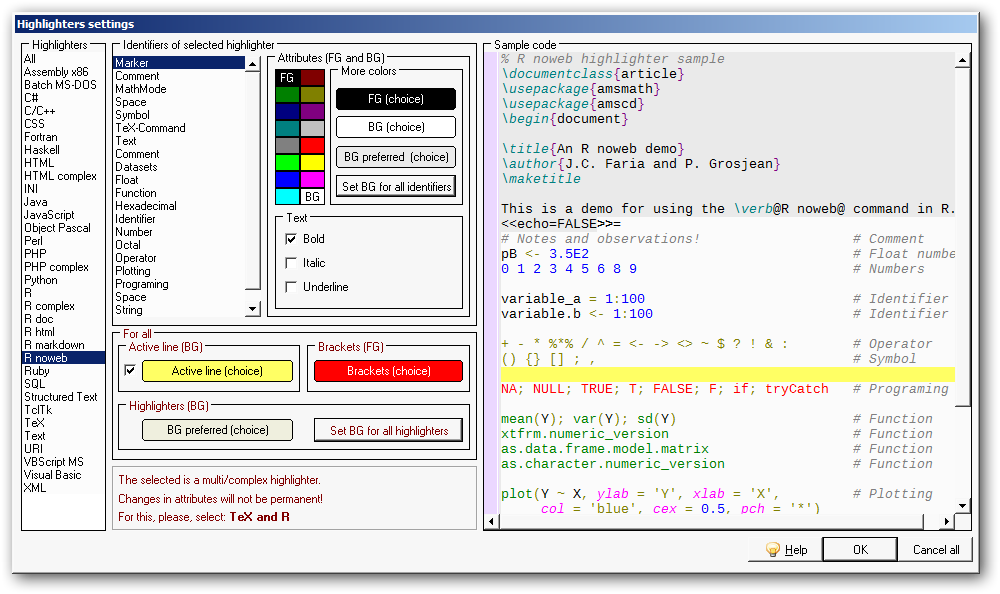
\includegraphics[scale=0.50]{./res/highlighter_settings.png}\\
  \caption{Highlighter preferences.}
  \label{fig:highlighter_preferences}
\end{figure}

This interface
(Figure \ref{fig:highlighter_preferences})
allows you to customize the appearance and colors of the
instances of the class \textit{SynEdit} (Editor, IO and LOG).

The interface is simple and self-explanatory.

Basically, make a choice between the set of highlighters available
from the \textit{Highlighters} list. The identifier of the selected
highlighter will be updated. It is possible to set only one
foreground attribute each time. But it is possible to set the
background for all attributes of the selected highlighter and also
the background of all attributes of all highlighters.

It is also possible to set the color brackets and the active line
background.


\subsubsection{Observation:}
\index{highlighters!multi-highlighters}

Tinn-R has seven multi-highlighters: \textit{HTML complex}, \textit{PHP complex},
\textit{R complex}, \textit{R doc},  \textit{R html}, \textit{R markdown} and \textit{R noweb},
with each one behaving as follows:

\begin{footnotesize}
  \begin{verbatim}
    1. HTML complex = HTML & JavaScript
    2. PHP complex  = HTML & JavaScript & PHP
    3. R complex    = R & URI ('<<<' begin URI; '>>>' end URI)
    4. R doc        = TeX & R ('>>=' begin R; '@' end R)
    5. R html       = HTML & R ('<!--begin.rcode' begin R; 'end.rcode-->' end R)
    5. R markdown   = URI & R ('```{' begin R; '```' end R)
    6. R noweb      = TeX & R ('>>=' begin R; '@' end R)

    URI       : Uniform Resource Identifiers.

    R complex : The main syntax is R, '<<<' and '>>>' are the tags enabling
                the user to insert a block of URI syntax.

    R doc     : The main syntax is TeX, '>>=' and '@' are the tags enabling
                the user to insert a block of R syntax.

    R html    : The main syntax is HTML, '<!--begin.rcode' and 'end.rcode-->' are the tags enabling
                the user to insert a block of R syntax.

    R markdown: The main syntax is URI, '```{' and '```' are the tags enabling
                the user to insert a block of R syntax.

    R noweb   : The main syntax is TeX, '>>=' and '@' are the tags enabling
                the user to insert a block of R syntax.

  \end{verbatim}
\end{footnotesize}

These highlighters haven't priorities when you set the syntax color preferences.
Thus, if you change the colors' preferences of any of these multi-highlighters
these settings will be valid only in the current Tinn-R session and will not be
saved when Tinn-R is closed. So, if you want to make permanent changes, set the
preferences from all simple highlighters.

From version 3.0.1.0 a warning message is displayed whenever
a multi-highlighter is selected. It shows which highlighters the user
must change the characteristics so that they are properly stored and
henceforth always displayed.
